\documentclass{article}
\usepackage[english]{babel}
\usepackage[letterpaper,top=2cm,bottom=2cm,left=2.5cm,right=2.5cm,marginparwidth=1.25cm]{geometry}

\usepackage[leqno]{amsmath}
\usepackage{enumitem, nccmath,lipsum,amssymb,xcolor,xparse,listings, blindtext, tikz, pgfplots}
\usepackage[most]{tcolorbox}

\NewDocumentCommand{\codeword}{v}{
\texttt{\textcolor{blue}{#1}}
}

\lstset{language=C, keywordstyle={\bfseries \color{blue}}}

\newcommand{\RN}[1]{%
  \textup{\uppercase\expandafter{\romannumeral#1}}%
}

\NewDocumentCommand{\mynote}{+O{}+m}{%
  \begingroup
  \tcbset{%
    noteshift/.store in=\mynote@shift,
    noteshift=1.5cm
  }
  \begin{tcolorbox}[nobeforeafter,
    enhanced,
    sharp corners,
    toprule=0.5pt,
    bottomrule=0.5pt,
    leftrule=0pt,
    rightrule=0pt,
    colback=green!10,
    #1,
    left skip=\mynote@shift,
    right skip=\mynote@shift,
    overlay={\node[right] (mynotenode) at ([xshift=-\mynote@shift]frame.west) {\textbf{Note:}} ;},
    ]
    #2
  \end{tcolorbox}
  \endgroup
  }
\makeatother

\newcommand{\mytext}[1]% #1 = same as intertext
{&\parbox{0.9\textwidth}{\rule{0pt}{.5\baselineskip}\\
\textrm{#1}\\
\rule{0pt}{.5\baselineskip}}&\\}

\newcounter{exercise}
\newcounter{problem}[exercise]
\newcommand{\myitem}{\stepcounter{problem}\tag*{\alph{problem})}}

\title{Differential Equations: Test 2 Preparation.}
\author{Mashenkov Timofei}
\begin{document}
\maketitle{}

\section*{Week 10.}

\subsection*{Task 961.}

\addtolength{\jot}{1pt}
\begin{fleqn}[1\parindent]
  \begin{gather*}
    y' = \frac{2x+y}{3x+4y} \\ 
    \frac{dy}{dx} = \frac{\frac{dy}{dt}}{\frac{dx}{dt}}; \begin{cases}
      \dot{y} = 2x+y \\ 
      \dot{x} = 3x+4y
    \end{cases} \\
    A = 
    \begin{bmatrix}
      3 & 4 \\ 
      2 & 1
    \end{bmatrix}
    \begin{pmatrix}
      x \\ y
    \end{pmatrix}
    = 
    \begin{pmatrix}
      \dot{x} \\ \dot{y}
    \end{pmatrix} \\ 
    \det{(A - I\lambda)} = 0 \\ 
    \begin{bmatrix}
      3-\lambda & 4 \\
      2 & 1-\lambda
    \end{bmatrix}
    = 0 = 3 - 3\lambda - \lambda + \lambda^2-8 = 0 \Rightarrow \begin{cases}
      \lambda_1 = 5 \\ \lambda_2 = -1 
    \end{cases} \\
  \end{gather*}
\end{fleqn}

\begin{itemize}
  \item A Stable knot. $\lambda_1 < \lambda_2 < 0$.
  \item An Unstable knot. $\lambda_1 > \lambda_2 > 0$.
  \item A saddle point. $\lambda_2 < 0 < \lambda_1$.
  \item An unstable line. $\lambda_1=0, \lambda_2>0$.
  \item A stable line. $\lambda_1<0, \lambda_2=0$.
\end{itemize}

\addtolength{\jot}{1pt}
\begin{fleqn}[1\parindent]
  \begin{gather*}
    \lambda_1 = 5 \\
    \begin{bmatrix}
      -2 & 4 \\ 2 & -4
    \end{bmatrix}
    \begin{pmatrix}
      x \\ y
    \end{pmatrix}
    = 
    \begin{pmatrix}
      0 \\ 0
    \end{pmatrix} \\
    \begin{cases}
      -2x + 4y = 0 \\
      x = 2y
    \end{cases} \rightarrow
    \lambda_1 = \begin{pmatrix}
      2 \\ 1
    \end{pmatrix} \\
    \lambda_2 = -1 \\
    \begin{bmatrix}
      4 & 4 \\ 2 & 2
    \end{bmatrix}
    \begin{pmatrix}
      x \\ y
    \end{pmatrix}
    =
    \begin{pmatrix}
      0 \\ 0
    \end{pmatrix} \\
    x + y = 0 \rightarrow \lambda_2 = \begin{pmatrix}
      1 \\ -1
    \end{pmatrix} 
  \end{gather*}
\end{fleqn}

\addtolength{\jot}{1pt}
\begin{fleqn}[1\parindent]
  \begin{gather*}
    x = 0: \\ 
    \begin{cases}
      \frac{dy}{dt} = y \\ 
      \frac{dx}{dt} = 4y
    \end{cases} \rightarrow
    \frac{dy}{dx} = \frac{1}{4} \\
    y = 0: \\ 
    \begin{cases}
      \frac{dy}{dt} = 2x \\ 
      \frac{dx}{dt} = 3x
    \end{cases} \rightarrow
    \frac{dy}{dx} = \frac{2}{3}
  \end{gather*}
\end{fleqn}

\addtolength{\jot}{1pt}
\begin{fleqn}[1\parindent]
  \begin{gather*}
    y' = \frac{2x+y}{3x+4y} \\
    \begin{cases}
      \dot{x} = 0 \\ 
      3x+4y=0
    \end{cases} \\ 
    y = \frac{3}{4}x \\ 
    \begin{cases}
      \dot{y} = 0
      2x+y=0
    \end{cases} \\
    y=-2x
  \end{gather*}
\end{fleqn}

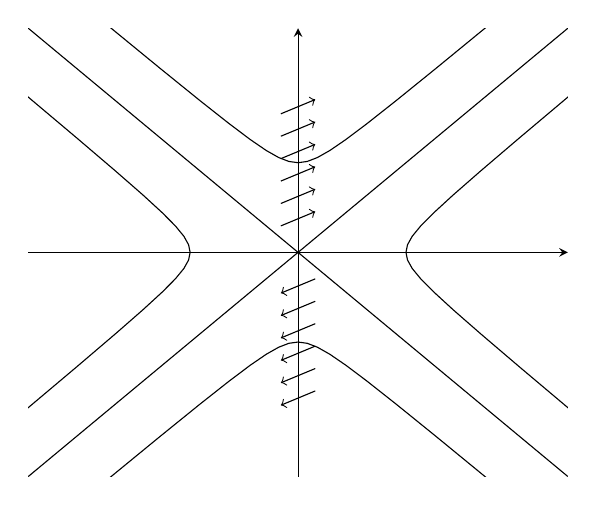
\begin{tikzpicture}
  \begin{axis}[xmin = -10, xmax = 10, ymin = -10, ymax = 10, axis x line=middle, axis y line=middle, ticks=none]
    \addplot[domain = -10:10] {x};
    \addplot[domain = -10:10] {-x};
    \addplot [domain=-4:4] ({cosh(x)+3}, {sinh(x)});
    \addplot [domain=-4:4] ({-cosh(x)-3}, {sinh(x)});
    \addplot [domain=-4:4] ({sinh(x)}, {cosh(x)+3});
    \addplot [domain=-4:4] ({sinh(x)}, {-cosh(x)-3});

    \node (s1) at (axis cs:-1,1){};
    \node (s2) at (axis cs:-1,2){};
    \node (s3) at (axis cs:-1,3){};
    \node (s4) at (axis cs:-1,4){};
    \node (s5) at (axis cs:-1,5){};
    \node (s6) at (axis cs:-1,6){};
    \node (d1) at (axis cs:1,2){};
    \node (d2) at (axis cs:1,3){};
    \node (d3) at (axis cs:1,4){};
    \node (d4) at (axis cs:1,5){};
    \node (d5) at (axis cs:1,6){};
    \node (d6) at (axis cs:1,7){};
    \draw[->](s1)--(d1);
    \draw[->](s2)--(d2);
    \draw[->](s3)--(d3);
    \draw[->](s4)--(d4);
    \draw[->](s5)--(d5);
    \draw[->](s6)--(d6);

    \node (sl1) at (axis cs:1,-1){};
    \node (sl2) at (axis cs:1,-2){};
    \node (sl3) at (axis cs:1,-3){};
    \node (sl4) at (axis cs:1,-4){};
    \node (sl5) at (axis cs:1,-5){};
    \node (sl6) at (axis cs:1,-6){};
    \node (dl1) at (axis cs:-1,-2){};
    \node (dl2) at (axis cs:-1,-3){};
    \node (dl3) at (axis cs:-1,-4){};
    \node (dl4) at (axis cs:-1,-5){};
    \node (dl5) at (axis cs:-1,-6){};
    \node (dl6) at (axis cs:-1,-7){};

    \draw[->](sl1)--(dl1);
    \draw[->](sl2)--(dl2);
    \draw[->](sl3)--(dl3);
    \draw[->](sl4)--(dl4);
    \draw[->](sl5)--(dl5);
    \draw[->](sl6)--(dl6);
  \end{axis}
\end{tikzpicture}

\subsection*{Task 848.}

\addtolength{\jot}{1pt}
\begin{fleqn}[1\parindent]
  \begin{gather*}
    \begin{cases}
      \dot{x} = -4x-2y+\frac{2}{e^t-1} \\ 
      \dot{y} = 6x+3y-\frac{3}{e^t-1}
    \end{cases} \\ 
    \begin{bmatrix}
      -4-\lambda & -2 \\ 
      \lambda & 3-\lambda
    \end{bmatrix} = 0 = -12+4\lambda-3\lambda+\lambda^2+12=0 \\ 
    \lambda^2+\lambda = 0 \\ 
    \lambda_1 = 0;\ \lambda_2 = -1 \\ \\ 
    \lambda_1 = 0: \\ 
    \begin{bmatrix}
      -4 & -2 \\ 6 & 3
    \end{bmatrix}
    \begin{pmatrix}
      x \\ y
    \end{pmatrix}
    =
    \begin{pmatrix}
      0 \\ 0
    \end{pmatrix} \\ 
    \begin{cases}
      -4x-2y=0 \\ 
      6x+3y=0
    \end{cases} \rightarrow 
    2x+y=0 \\ 
    x = 1;\ y=-2 \\ 
    \lambda_1 = \begin{pmatrix}
      1 \\ -2
    \end{pmatrix} \\ \\
    \lambda_2 = -1: \\
    \begin{bmatrix}
      -3 & -2 \\ 6 & 4
    \end{bmatrix}
    \begin{pmatrix}
      x \\ y
    \end{pmatrix}
    =
    \begin{pmatrix}
      0 \\ 0
    \end{pmatrix} \\ 
    -3x-2y=0 \\ 
    \begin{mmatrix}
      x = 2 \\ 
      y = -3 
    \end{mmatrix} \rightarrow \lambda_2 = 
    \begin{pmatrix}
      2 \\ -3
    \end{pmatrix} \\ 
  \end{gather*}
\end{fleqn}

\addtolength{\jot}{1pt}
\begin{fleqn}[1\parindent]
  \begin{gather*}
    \begin{pmatrix}
      x_0 \\ y_0
    \end{pmatrix} = 
    c_1(t) \cdot \begin{pmatrix}
      1 \\ -2
    \end{pmatrix}
    \cdot e^{0\cdot t} + c_2(t) \cdot \begin{pmatrix}
      2 \\ -3
    \end{pmatrix}
    \cdot e^{-1\cdot t} \\
    \begin{cases}
      c_1'(t)+2c_2'(t)e^{-t}=\frac{2}{e^t-1} \\
      -2c_1'(t)-3c_2'(t)e^{-1t}=-\frac{3}{e^t-1}
    \end{cases} \\ 
    c_2'(t)e^{-t}=\frac{1}{e^t-1}\\
    c_2'(t)=\frac{e^t}{e^t-1} \rightarrow
    c_2(t)=\int{\frac{e^t}{e^t-1}dt} \\ 
    e^t = v;\ dte^t = dv;\ dt = \frac{dv}{e^t} \\ 
    \int{\frac{1}{e^t}\frac{e^t}{v-1}dv} \rightarrow
    \ln{(|e^t-1|)}+\bar c_2 \\ 
    c_1'(t)+\frac{2e^t}{e^t-1}e^t=\frac{2}{e^t-1}\rightarrow
    \begin{matrix}
      c_1(t) = 0 \\ c_1(t) = \bar c_1
    \end{matrix}
  \end{gather*}
\end{fleqn}

\subsection*{Task 795.}

\addtolength{\jot}{1pt}
\begin{fleqn}[1\parindent]
  \begin{gather*}
    \begin{cases}
      \dot{x}=5x+3y\\ 
      \dot{y}=-3x-y
    \end{cases} \\ 
    \begin{bmatrix}
      5-\lambda & 3 \\ -3 & -1-\lambda
    \end{bmatrix}
    = 0 = -5-5\lambda-\lambda+\lambda^2+9=0 \\ 
    \lambda^2-4\lambda+4 = 0 \\ 
    \lambda_{1,2}=2 \\ 
    \RN{1}.\\ 
    \begin{cases}
      x=(ax+b)e^2t \\ 
      y=(cx+d)e^2t 
    \end{cases} \\ 
    ae^{2t}+2t+ae^{2t}+2be^{2t} = 5e^{2t}at+5e^{2t}b+3cte^{2t}+3e^{2t}d \rightarrow 
    \begin{cases}
      a+2b=5b+3d \\ 
      2a=5a+3c
    \end{cases} \\ 
    \RN{2}. \\
    \begin{bmatrix}
      3&3\\-3&-3
    \end{bmatrix}
    \begin{pmatrix}
      x\\y
    \end{pmatrix}
    =
    \begin{pmatrix}
      0\\0
    \end{pmatrix}\\ 
    \begin{matrix}
      3x+3y=0\\ 
      x=-y
    \end{matrix} \rightarrow 
    \begin{pmatrix}
      -1 \\ 1
    \end{pmatrix} \\ 
    \begin{bmatrix}
      3&3\\-3&-3
    \end{bmatrix}
    \begin{pmatrix}
      x\\y
    \end{pmatrix}
    =
    \begin{pmatrix}
      -1\\1
    \end{pmatrix} \\ 
    \begin{matrix}
      3x+3y=-1 & -3x-3y=1\\ 
      x=1;\ y = -\frac{4}{3} & x=1;\ y=-\frac{4}{3}
    \end{matrix} \rightarrow 
    \begin{pmatrix}
      1 \\ -\frac{4}{3}
    \end{pmatrix}
  \end{gather*}
\end{fleqn}

\addtolength{\jot}{1pt}
\begin{fleqn}[1\parindent]
  \begin{gather*}
    \begin{pmatrix}
      x\\y
    \end{pmatrix} = 
    c_1 
    \begin{pmatrix}
      -1\\1
    \end{pmatrix}
    e^{2t}+c_2e^{2t}
    \Bigg(t\cdot\begin{pmatrix}
      -1\\1
    \end{pmatrix}
    +
    \begin{pmatrix}
      1\\-\frac{4}{3}
    \end{pmatrix}\Bigg)
  \end{gather*}
\end{fleqn}

\subsection*{Task 797.}

\addtolength{\jot}{1pt}
\begin{fleqn}[1\parindent]
  \begin{gather*}
    \begin{cases}
      \dot{x}=x-2y-z \\ 
      \dot{y}=y-x+z \\ 
      \dot{x}=x-1
    \end{cases}\ (\lambda_1=0,\ \lambda_2=2,\ \lambda_3=-1). \\ 
    A =
    \begin{bmatrix}
      1-\lambda&-2&-1 \\ 
      -1 & 1-\lambda & 1 \\ 
      1 & 0 & -1-\lambda
    \end{bmatrix} \\ 
    \lambda_1 = 0 \\ 
    \begin{bmatrix}
      1 & -2 & -1 \\ 
      -1 & 1 & 1 \\ 
      1 & 0 & -1
    \end{bmatrix}
    \begin{pmatrix}
      x \\ y \\ z
    \end{pmatrix}
    =
    \begin{pmatrix}
      0 \\ 0 \\ 0
    \end{pmatrix} \\ 
    \begin{bmatrix}
      1 & -2 & -1 \\
      -1 & 1 & 1 \\
      1 & 0 & -1
    \end{bmatrix} \xrightarrow{\text{RREF}} \begin{bmatrix}
      1 & 0 & -1 \\ 
      0 & -1 & 0 \\ 
      0 & 0 & 0
    \end{bmatrix}
    \begin{pmatrix}
      x \\ y \\ z
    \end{pmatrix} = \begin{pmatrix}
      0 \\ 0 \\ 0
    \end{pmatrix} \\ 
    \begin{cases}
      x-2=0 \\ 
      -y=0
    \end{cases} \rightarrow
    \lambda_1: \begin{pmatrix}
      1 \\ 0 \\ 1
    \end{pmatrix} \\
    \lambda_2: \begin{pmatrix}
      3 \\ -2 \\ 1
    \end{pmatrix} \\ 
    \lambda_3: \begin{pmatrix}
      0 \\ -1 \\ 2
    \end{pmatrix} \\ 
    \begin{pmatrix}
      x \\ y \\ z
    \end{pmatrix} = 
    \begin{pmatrix}
      c_1e^{0t}\cdot1+c_2e^{2t}\cdot 3+c_3e^{-1t}\cdot 0 \\ 
      c_1e^{0t}\cdot0+c_2e^{2t}\cdot (-2)+c_3e^{-1t}\cdot (-1) \\
      c_1e^{0t}\cdot1+c_2e^{2t}\cdot 1+c_3e^{-1t}\cdot 2
    \end{pmatrix}
  \end{gather*}
\end{fleqn}

\subsection*{Task 967.}

\addtolength{\jot}{1pt}
\begin{fleqn}[1\parindent]
  \begin{gather*}
    \begin{cases}
      \dot{x}=-3x+2y\\ 
      \dot{y}=-2x+y
    \end{cases} \\ 
    \begin{vmatrix}
      -3-\lambda & 2 \\ 
      -2 & 1-\lambda
    \end{vmatrix}
    = 0 = -3+3\lambda-\lambda+\lambda^2+4=0 \\ 
    \lambda^2+2\lambda+1 = 0 \\ 
    \lambda_{1,2}=-1 \rightarrow \begin{pmatrix}
      1 \\ 1
    \end{pmatrix} \\
    x = 0: \\ 
    \begin{cases}
      \dot{x} = 2y \\ 
      \dot{y} = y 
    \end{cases} \rightarrow
    \frac{dy}{dx} = \frac{1}{2} \\ 
    y = 0: \\ 
    \begin{cases}
      \dot{x} = -3x \\ 
      \dot{y} = -2x
    \end{cases} \rightarrow
    \frac{dy}{dx} = \frac{2}{3} \\ 
    \begin{cases}
      \dot{x} = 0\\
      -3x+2y=0\\
    \end{cases}
    \begin{cases}
      \dot{y}=0\\ 
      -2x+y=0
    \end{cases} \\ 
    y = \frac{3x}{2}\ y =2x \\ 
  \end{gather*}
\end{fleqn}

I don't know how to plot this :(

\end{document}
